% !TEX program = xelatex
% 需要的宏包：ctex, amsmath, amssymb, xcolor, tikz, pgfplots
\documentclass[UTF8]{ctexart}

\usepackage{amsmath,amssymb}
\usepackage[a4paper,margin=18mm]{geometry}
\usepackage{xcolor}
\usepackage{tikz}
\usepackage{pgfplots}
\pgfplotsset{compat=1.18}

\setlength{\parindent}{2em}
\setlength{\parskip}{0.4em}

\usepackage{tikz}
\usetikzlibrary{calc}


\begin{document}
	
	\begin{center}
		{\LARGE\bfseries\color{red}{抛物线与阿基米德三角形}}
	\end{center}
	
	\section*{\color{blue}{阿基米德三角形}}
	
	\textbf{\color{purple}{定义：}}
	抛物线的弦与过弦的端点的两条切线所围成的三角形叫做阿基米德三角形，如下图 $\triangle ABM$ 即为阿基米德三角形。
	记弦 $AB$ 为阿基米德三角形 $\triangle ABM$ 的底，
	$A(x_1,y_1)$，$B(x_2,y_2)$。
	
	下文默认抛物线为
	\[
	y^2=2px\quad(p>0),
	\]
	其焦点为 $F\!\left(\dfrac p2,0\right)$，准线为 $x=-\dfrac p2$，轴为 $x$ 轴。
	
	\begin{figure}[h]
		\centering
		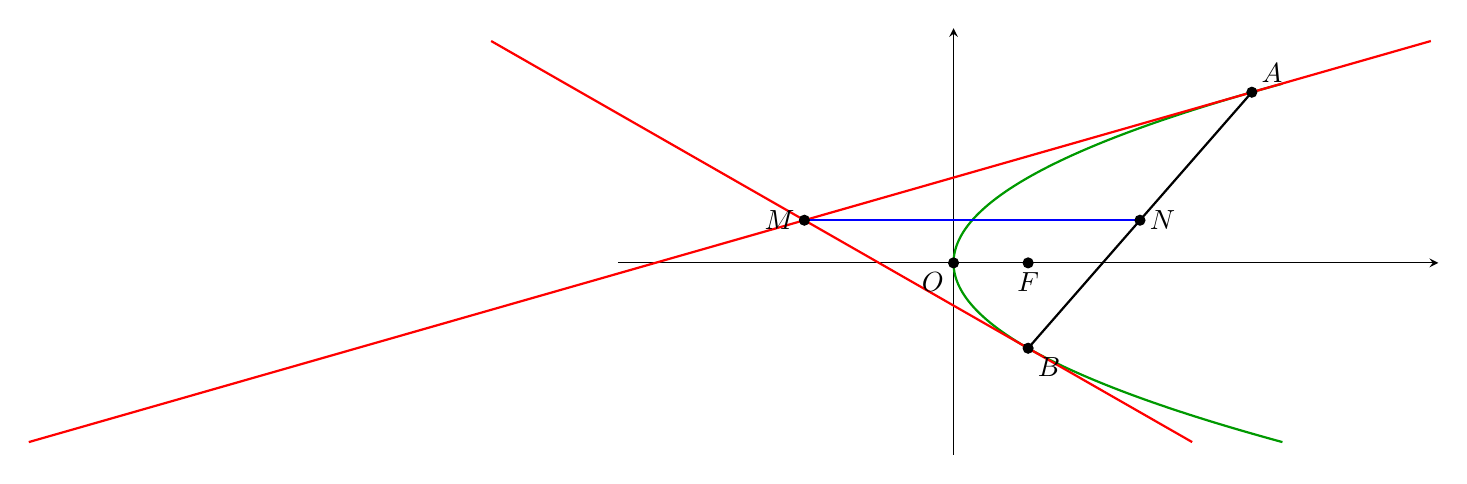
\begin{tikzpicture}
			\begin{axis}[
				axis lines=middle,
				xmin=-4.5, xmax=6.5,
				ymin=-4.5, ymax=5.5,
				xtick=\empty, ytick=\empty,
				width=12cm, height=7cm,
				clip=false
				]
				% 取示意参数：p=2，则 y^2=4x
				% 抛物线：x = y^2/4
				\addplot[domain=-4.2:4.2,samples=220,thick,green!60!black]
				({x^2/4},{x});
				
				% 取点：A(4,4), B(1,-2)
				\addplot[thick] coordinates {(4,4) (1,-2)}; % chord AB
				% 切线：A 对应参数 t=2: 2y = x+4 -> x=2y-4
				\addplot[domain=-4.2:5.2,samples=2,thick,red]
				({2*x-4},{x});
				% 切线：B 对应参数 t=-1: -y = x+1 -> x=-y-1
				\addplot[domain=-4.2:5.2,samples=2,thick,red]
				({-x-1},{x});
				
				% 交点 M = (t1 t2, t1+t2)=(-2,1)，中点 N=(2.5,1)
				\addplot[thick,blue] coordinates {(-2,1) (2.5,1)}; % MN // x-axis
				
				% 关键点
				\addplot[only marks,mark=*,mark size=1.8pt]
				coordinates {(0,0) (1,0) (4,4) (1,-2) (-2,1) (2.5,1)};
				\node[below left] at (axis cs:0,0) {$O$};
				\node[below]      at (axis cs:1,0) {$F$};
				\node[above right]at (axis cs:4,4) {$A$};
				\node[below right]at (axis cs:1,-2) {$B$};
				\node[left]       at (axis cs:-2,1) {$M$};
				\node[right]      at (axis cs:2.5,1) {$N$};
				
			\end{axis}
		\end{tikzpicture}
		\caption{阿基米德三角形示意图（取 $p=2$ 作图）}
	\end{figure}
	
	\section*{\color{purple}{主要性质：}}
	
	\subsection*{\color{green!60!black}{性质 1}}
	阿基米德三角形底边上的中线平行于抛物线的轴，如上图 $NM\parallel x$ 轴。
	
	\textbf{\color{red}{证明：}}
	设 $N$ 为弦 $AB$ 中点，则过 $A$ 的切线方程为
	\[
	y_1y=p(x+x_1),
	\]
	过 $B$ 的切线方程为
	\[
	y_2y=p(x+x_2).
	\]
	联立方程组
	\[
	\begin{cases}
		y_1y=p(x+x_1),\\
		y_2y=p(x+x_2),
	\end{cases}
	\qquad \text{又}\qquad
	\begin{cases}
		y_1^{\,2}=2px_1,\\
		y_2^{\,2}=2px_2,
	\end{cases}
	\]
	解得两切线交点
	\[
	M\!\left(\dfrac{y_1y_2}{2p},\ \dfrac{y_1+y_2}{2}\right),
	\]
	进而可知 $NM\parallel x$ 轴。
	
	\subsection*{\color{green!60!black}{性质 2}}
	底边长为 $a$ 的阿基米德三角形的面积的最大值为
	\[
	\frac{a^3}{8p}.
	\]
	
	\textbf{\color{red}{证明：}}
	$|AB|=a$，设 $M$ 到 $AB$ 的距离为 $d$，由性质 1 知，
	\[
	d\le |MN|
	=\frac{x_1+x_2}{2}-\frac{y_1y_2}{2p}
	=\frac{y_1^2+y_2^2}{4p}-\frac{y_1y_2}{2p}
	=\frac{(y_1-y_2)^2}{4p}.
	\]
	设直线 $AB$ 的方程为 $x=my+n$，则
	\[
	a=\sqrt{(1+m^2)(y_1-y_2)^2}.
	\]
	所以 $(y_1-y_2)^2\le a^2$，即
	\[
	d\le \frac{a^2}{4p}.
	\]
	所以
	\[
	S_{\triangle ABM}=\frac12ad\le \frac{a^3}{8p}.
	\]
	证毕。
	
	\textbf{\color{red}{特别地：}}
	若阿基米德三角形的底边过焦点，则顶点 $M$ 的轨迹为准线，
	且阿基米德三角形的面积的最小值为 $p^2$。
	
	\subsection*{\color{green!60!black}{性质 3}}
	在阿基米德三角形中，
	\[
	\angle MFA=\angle MFB.
	\]
	
	\begin{figure}[h]
		\centering
		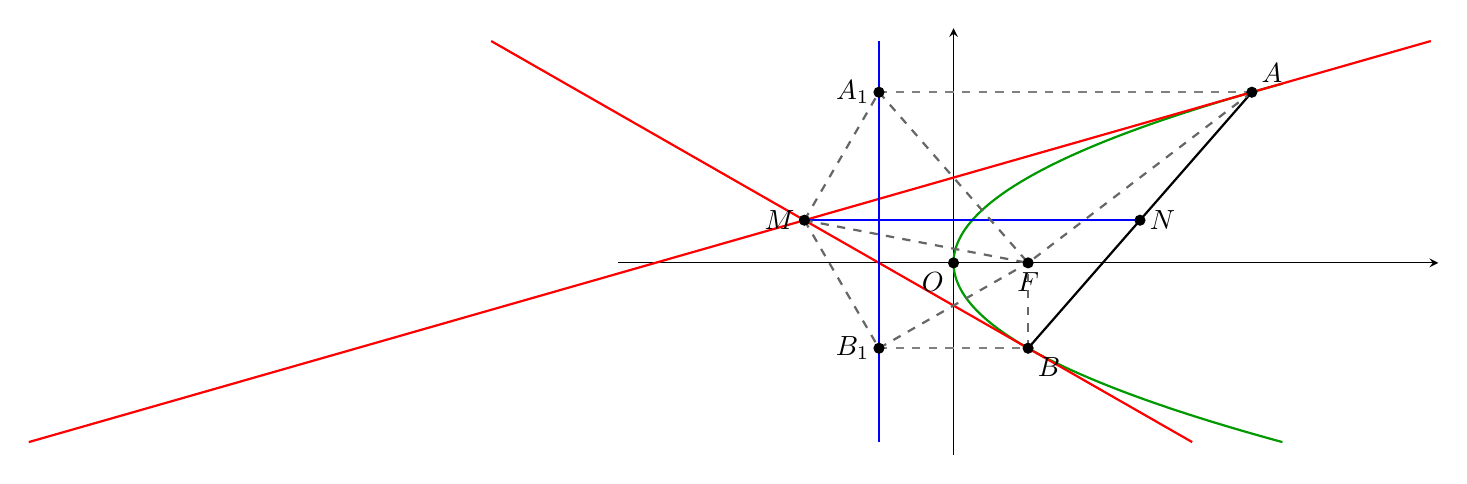
\begin{tikzpicture}
			\begin{axis}[
				axis lines=middle,
				xmin=-4.5, xmax=6.5,
				ymin=-4.5, ymax=5.5,
				xtick=\empty, ytick=\empty,
				width=12cm, height=7cm,
				clip=false
				]
				% 抛物线 y^2=4x
				\addplot[domain=-4.2:4.2,samples=220,thick,green!60!black]
				({x^2/4},{x});
				
				% chord and tangents
				\addplot[thick] coordinates {(4,4) (1,-2)}; % AB
				\addplot[domain=-4.2:5.2,samples=2,thick,red] ({2*x-4},{x}); % tangent at A
				\addplot[domain=-4.2:5.2,samples=2,thick,red] ({-x-1},{x}); % tangent at B
				
				% points
				\addplot[only marks,mark=*,mark size=1.8pt]
				coordinates {(0,0) (1,0) (4,4) (1,-2) (-2,1) (2.5,1) (-1,4) (-1,-2)};
				\node[below left] at (axis cs:0,0) {$O$};
				\node[below]      at (axis cs:1,0) {$F$};
				\node[above right]at (axis cs:4,4) {$A$};
				\node[below right]at (axis cs:1,-2) {$B$};
				\node[left]       at (axis cs:-2,1) {$M$};
				\node[right]      at (axis cs:2.5,1) {$N$};
				\node[left]       at (axis cs:-1,4) {$A_1$};
				\node[left]       at (axis cs:-1,-2) {$B_1$};
				
				% MN
				\addplot[thick,blue] coordinates {(-2,1) (2.5,1)};
				
				% directrix x=-1 (p=2 -> x=-p/2=-1)
				\addplot[thick,blue] coordinates {(-1,-4.2) (-1,5.2)};
				
				% perpendiculars to directrix: AA1 and BB1 (dashed)
				\addplot[dashed,thick,gray] coordinates {(-1,4) (4,4)};
				\addplot[dashed,thick,gray] coordinates {(-1,-2) (1,-2)};
				
				% auxiliary segments (dashed)
				\addplot[dashed,thick,black!60] coordinates {(-2,1) (-1,4)};   % MA1
				\addplot[dashed,thick,black!60] coordinates {(-2,1) (-1,-2)};  % MB1
				\addplot[dashed,thick,black!60] coordinates {(-2,1) (1,0)};    % MF
				\addplot[dashed,thick,black!60] coordinates {(4,4) (1,0)};     % AF
				\addplot[dashed,thick,black!60] coordinates {(1,-2) (1,0)};    % BF
				\addplot[dashed,thick,black!60] coordinates {(-1,4) (1,0)};    % A1F
				\addplot[dashed,thick,black!60] coordinates {(-1,-2) (1,0)};   % B1F
				
			\end{axis}
		\end{tikzpicture}
		\caption{性质 3 的几何关系示意图（取 $p=2$ 作图）}
	\end{figure}
	
	\textbf{\color{red}{证明：}}
	如下图，过点 $A,B$ 分别作抛物线准线的垂线 $AA_1,BB_1$，垂足为 $A_1,B_1$，
	连接 $A_1M,B_1M,MF,AF,BF,A_1F,B_1F$，则
	\[
	k_{FA_1}=-\frac{y_1}{p},\qquad k_{MA}=\frac{p}{y_1},
	\]
	从而
	\[
	k_{MA}\cdot k_{FA_1}=-1,
	\]
	所以 $FA_1\perp MA$。
	
	由抛物线定义，得 $|AA_1|=|FA|$，
	由此可知 $MA$ 是线段 $FA_1$ 的中垂线，得到
	\[
	|MA_1|=|MF|,\qquad \angle MA_1A=\angle MFA.
	\]
	同理可证
	\[
	|MB_1|=|MF|,\qquad \angle MB_1B=\angle MFB.
	\]
	所以
	\[
	|MA_1|=|MF|=|MB_1|,
	\]
	即
	\[
	\angle MA_1B_1=\angle MB_1A_1.
	\]
	因为
	\[
	\angle MA_1A=\angle MA_1B_1+90^\circ,\qquad
	\angle MB_1B=\angle MB_1A_1+90^\circ,
	\]
	所以
	\[
	\angle MA_1A=\angle MB_1B,
	\]
	即
	\[
	\angle MFA=\angle MFB.
	\]
	
	\textbf{\color{red}{特别的：}}
	若阿基米德三角形的底边过焦点，此时 $\angle MFA=\angle MFB$，
	即 $MF\perp AB$。
	
	\subsection*{\color{green!60!black}{性质 4}}
	\[
	|AF|\cdot|BF|=|MF|^2.
	\]
	
	\textbf{\color{red}{证明：}}
	\[
	|AF|\cdot|BF|
	=\left(x_1+\frac p2\right)\left(x_2+\frac p2\right)
	=x_1x_2+\frac p2(x_1+x_2)+\frac{p^2}{4}.
	\]
	将
	\[
	\begin{cases}
		y_1^2=2px_1,\\
		y_2^2=2px_2
	\end{cases}
	\]
	代入得：
	\[
	|AF|\cdot|BF|
	=\frac{y_1^2y_2^2}{4p^2}+\frac{y_1^2+y_2^2}{4}+\frac{p^2}{4}.
	\]
	由性质 1 可知：
	\[
	M\!\left(\frac{y_1y_2}{2p},\ \frac{y_1+y_2}{2}\right),\qquad
	F\!\left(\frac p2,0\right),
	\]
	则有
	\begin{align*}
		|MF|^2
		&=\left(\frac{y_1y_2}{2p}-\frac p2\right)^2+\left(\frac{y_1+y_2}{2}\right)^2\\
		&=\frac{y_1^2y_2^2}{4p^2}+\frac{y_1^2+y_2^2}{4}+\frac{p^2}{4}.
	\end{align*}
	所以
	\[
	|AF|\cdot|BF|=|MF|^2.
	\]
	证毕。
	
	
	%====================（续：底边 AB 过焦点的阿基米德三角形）====================
	% 需要的宏包（按需加入你的导言区）：
	% \usepackage{amsmath,amssymb}
	% \usepackage{xcolor}
	% \usepackage{tikz}
	% \usepackage{pgfplots}
	% \pgfplotsset{compat=1.18}
	
	\section*{重点：底边 $AB$ 过焦点的阿基米德三角形特殊性质}
	
	\subsection{\textcolor{purple}{辨识}：特殊的阿基米德三角形（对三个顶点的确定）}

	\textbf{对于点 $A,B$：}
	\begin{enumerate}
		\item[(1)] 抛物线\textbf{焦点弦}与抛物线的交点；
		\item[(2)] 由准线上一点向抛物线引两条切线所对应的切点。
	\end{enumerate}
	
	\textbf{对于点 $M$：}
	\begin{enumerate}
		\item[(3)] 过焦点弦的一个端点所作的切线与准线的交点；
		\item[(4)] 过焦点弦的两个端点所作两条切线的交点。
	\end{enumerate}
	
	满足以上 $(1)(3)$ 或 $(1)(4)$ 或 $(2)(3)$ 或 $(2)(4)$ 的三个点所组成的三角形
	即为\textbf{“底边过焦点的阿基米德三角形”}。
	


	
	\subsection{\textcolor{purple}{主要性质}}
	
	我们归纳底边 $AB$ 过焦点的阿基米德三角形特殊性质如下（设抛物线为 $y^2=2px$，焦点 $F\!\left(\frac p2,0\right)$，准线为 $x=-\frac p2$）：
	
	\begin{figure}[htbp]
		\centering
		\resizebox{0.5\linewidth}{!}{%
		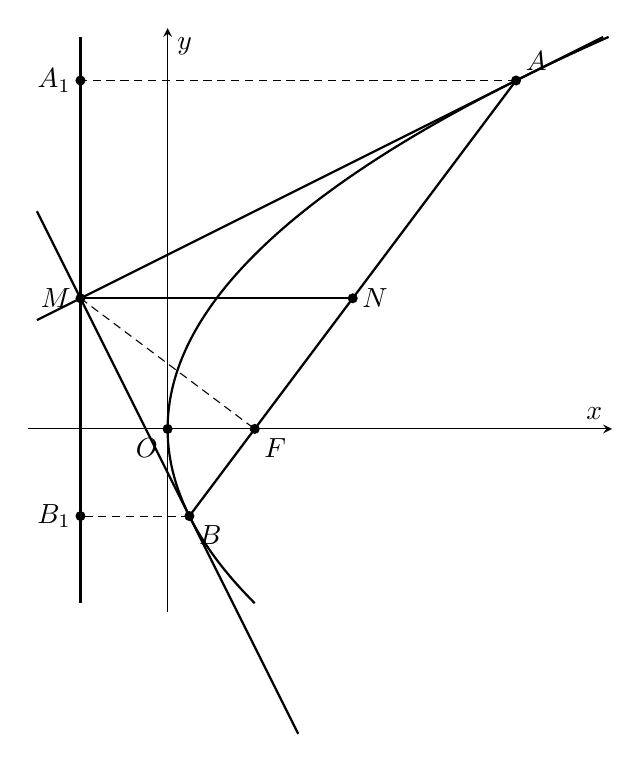
\begin{tikzpicture}
			\begin{axis}[
				axis lines=middle,
				axis equal image,
				xmin=-3.2,xmax=10.2,
				ymin=-4.2,ymax=9.2,
				xlabel={$x$}, ylabel={$y$},
				ticks=none,
				width=0.86\linewidth,
				clip=false
				]
				% 取示意抛物线 y^2=8x（即 p=4）
				\addplot[domain=-4:9,samples=300,thick] ({x^2/8},{x});
				
				% 准线 x=-2
				\addplot[domain=-4:9,samples=2,thick] ({-2},{x});
				
				% 关键点（示意取参数 t=2 的焦点弦端点）
				% A=(8,8), B=(0.5,-2), F=(2,0), M=T=(-2,3), N=(4.25,3), A1=(-2,8), B1=(-2,-2), O=(0,0)
				\addplot[only marks,mark=*,mark size=1.6pt] coordinates
				{(8,8) (0.5,-2) (2,0) (-2,3) (4.25,3) (-2,8) (-2,-2) (0,0)};
				
				\node[above right] at (axis cs:8,8) {$A$};
				\node[below right] at (axis cs:0.5,-2) {$B$};
				\node[below right] at (axis cs:2,0) {$F$};
				\node[left]       at (axis cs:-2,3) {$M$};
				\node[right]      at (axis cs:4.25,3) {$N$};
				\node[left]       at (axis cs:-2,8) {$A_1$};
				\node[left]       at (axis cs:-2,-2) {$B_1$};
				\node[below left] at (axis cs:0,0) {$O$};
				
				% 焦点弦 AB
				\addplot[thick] coordinates {(8,8) (0.5,-2)};
				
				% 两端点处切线（t=2: y=x/2+4；t=-1/2: y=-2x-1）
				\addplot[thick] coordinates {(-3,2.5) (10,9)};      % y = x/2 + 4
				\addplot[thick] coordinates {(-3,5) (3,-7)};        % y = -2x - 1
				
				% MN // x 轴
				\addplot[thick] coordinates {(-2,3) (4.25,3)};
				
				% AA1, BB1（与 x 轴平行）
				\addplot[densely dashed] coordinates {(8,8) (-2,8)};
				\addplot[densely dashed] coordinates {(0.5,-2) (-2,-2)};
				
				% A1B1（在准线上）
				\addplot[densely dashed] coordinates {(-2,8) (-2,-2)};
				
				% MF（性质2 用）
				\addplot[densely dashed] coordinates {(-2,3) (2,0)};
				
			\end{axis}
		\end{tikzpicture}
	}
		\caption{底边过焦点的阿基米德三角形示意图（取 $y^2=8x$，即 $p=4$ 作图）}
	\end{figure}
	
	\paragraph{\textcolor{green!60!black}{性质1：}}
	顶点 $M$ 的坐标为
	\[
	M\left(-\frac{p}{2},\ \frac{y_1+y_2}{2}\right).
	\]
	即顶点 $M$ 的轨迹为准线；底边上的中线平行于抛物线上的轴（$MN$ 平行于 $x$ 轴）。
	
	\paragraph{\textcolor{green!60!black}{性质2：}}
	如上图，$MF\perp AB$。
	
	\paragraph{\textcolor{red}{证明：}}
	\[
	M\left(-\frac{p}{2},\ \frac{y_1+y_2}{2}\right),\quad F\left(\frac{p}{2},0\right),
	\]
	则
	\[
	\overrightarrow{MF}=\left(p,-\frac{y_1+y_2}{2}\right).
	\]
	则
	\[
	\overrightarrow{AB}\cdot\overrightarrow{MF}
	=(x_2-x_1,\ y_1-y_2)\cdot\left(p,-\frac{y_1+y_2}{2}\right)
	= p(x_2-x_1)+\frac{y_1^2-y_2^2}{2},
	\]
	又 $A(x_1,y_1),\ B(x_2,y_2)$ 在抛物线 $y^2=2px$ 上，所以
	\[
	x_1=\frac{y_1^2}{2p},\quad x_2=\frac{y_2^2}{2p},
	\]
	因此
	\[
	\overrightarrow{AB}\cdot\overrightarrow{MF}
	= p\!\left(\frac{y_2^2}{2p}-\frac{y_1^2}{2p}\right)+\frac{y_1^2-y_2^2}{2}=0,
	\]
	即 $MF\perp AB$。
	
	\paragraph{\textcolor{green!60!black}{性质3：}}
	如上图，$MA\perp MB$。
	
	\paragraph{\textcolor{red}{证明：}}
	$MN$ 是梯形的中位线，则有
	\[
	|AB|=|AF|+|BF|=|AA_1|+|BB_1|=2|MN|,
	\]
	因此以 $AB$ 为直径的圆与准线相切，切点为 $M$；因此直径 $AB$ 所对的圆周角
	\[
	\angle AMB=\frac{\pi}{2},
	\]
	即 $MA\perp MB$。
	
	\paragraph{\textcolor{green!60!black}{性质4：}}
	阿基米德三角形的面积的最小值为 $p^2$。
	
	\paragraph{\textcolor{red}{证明：}}
	设焦点弦 $AB$ 所在直线的倾斜角为 $\alpha$，
	
	由性质2可知，$MF$ 为 $\triangle ABM$ 的高，所以
	\[
	S_{\triangle ABM}=\frac12\cdot|AB|\cdot|MF|.
	\]
	
	由 $AA_1\parallel x$ 轴可得：$\angle A_1FO=\angle FA_1A$。
	
	由 $|AF|=|AA_1|$ 可得：
	\[
	\angle FA_1A=\angle A_1FA,
	\]
	因此
	\[
	\angle A_1FO=\angle A_1FA=\frac12\angle AFO.
	\]
	
	同理可得：
	\[
	\angle B_1FO=\frac12\angle BFO,
	\]
	所以
	\[
	\angle A_1FB_1=\angle A_1FO+\angle B_1FO
	=\frac12\angle AFO+\frac12\angle BFO=\frac{\pi}{2}.
	\]
	
	所以 $\triangle A_1FB_1$ 为直角三角形，由斜边中线等于斜边一半可得：
	\[
	|MF|=\frac12|A_1B_1|.
	\]
	因此
	\[
	|MF|=\frac12|A_1B_1|=\frac12\cdot|AB|\cdot\sin\alpha,
	\]
	所以
	\[
	S_{\triangle ABC_1}
	=\frac12\cdot|AB|\times \frac12\cdot|AB|\cdot\sin\alpha
	=\frac14|AB|^2\sin\alpha.
	\]
	
	由焦半径倾斜角公式可知，
	\[
	|AB|=|AF|+|BF|
	=\frac{p}{1-\cos\alpha}+\frac{p}{1+\cos\alpha}
	=\frac{p(1+\cos\alpha)+p(1-\cos\alpha)}{1-\cos^2\alpha}
	=\frac{2p}{\sin^2\alpha}.
	\]
	所以
	\[
	S_{\triangle ABC_1}
	=\frac14\left(\frac{2p}{\sin^2\alpha}\right)^2\sin\alpha
	=\frac{p^2}{\sin^3\alpha},
	\]
	又因为 $\sin^3\alpha\le 1$，所以阿基米德三角形 $ABM$ 面积的最小值为 $p^2$。
	
	\*section{（精选例题）}
	
	\paragraph{例1.}
	已知直线 $l$ 与抛物线 $C: y^2=8x$ 相切于点 $P$，且与 $C$ 的准线相交于点 $T$，$F$ 为 $C$ 的焦点，
	连接 $PF$ 交 $C$ 于另一点 $Q$，则 $\triangle PTQ$ 面积的最小值为\underline{\qquad}；
	若 $|TF|=5$，则 $|PQ|$ 的值为\underline{\qquad}。（本小题第一空 2 分，第二空 3 分）
	
	\begin{figure}[htbp]
		\centering
		\resizebox{0.5\linewidth}{!}{%
		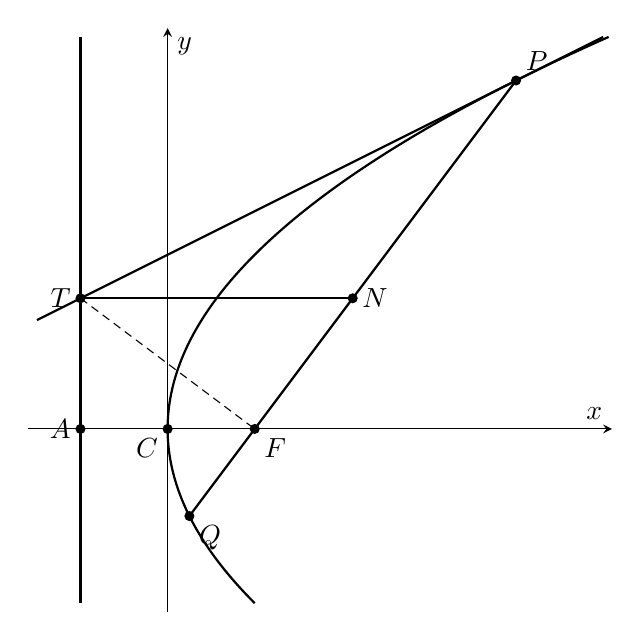
\begin{tikzpicture}
			\begin{axis}[
				axis lines=middle,
				axis equal image,
				xmin=-3.2,xmax=10.2,
				ymin=-4.2,ymax=9.2,
				xlabel={$x$}, ylabel={$y$},
				ticks=none,
				width=0.86\linewidth,
				clip=false
				]
				% 抛物线 y^2=8x
				\addplot[domain=-4:9,samples=300,thick] ({x^2/8},{x});
				
				% 准线 x=-2
				\addplot[domain=-4:9,samples=2,thick] ({-2},{x});
				
				% 取 P 对应参数 t=2：P(8,8)，Q 对应 -1/t：Q(0.5,-2)，F(2,0)，T(-2,3)
				\addplot[only marks,mark=*,mark size=1.6pt] coordinates
				{(8,8) (0.5,-2) (2,0) (-2,3) (4.25,3) (-2,0) (0,0)};
				
				\node[above right] at (axis cs:8,8) {$P$};
				\node[below right] at (axis cs:0.5,-2) {$Q$};
				\node[below right] at (axis cs:2,0) {$F$};
				\node[left]       at (axis cs:-2,3) {$T$};
				\node[right]      at (axis cs:4.25,3) {$N$};
				\node[left]       at (axis cs:-2,0) {$A$};
				\node[below left] at (axis cs:0,0) {$C$};
				
				% 切线 l：t=2 => y=x/2+4
				\addplot[thick] coordinates {(-3,2.5) (10,9)};
				
				% 焦点弦 PQ
				\addplot[thick] coordinates {(8,8) (0.5,-2)};
				
				% 连接 PF
				\addplot[densely dashed] coordinates {(2,0) (8,8)};
				
				% 连接 TF
				\addplot[densely dashed] coordinates {(-2,3) (2,0)};
				
				% TN // x 轴（性质1中的中线）
				\addplot[thick] coordinates {(-2,3) (4.25,3)};
				
			\end{axis}
		\end{tikzpicture}
	}
		\caption{例1示意图（$C:y^2=8x$）}
	\end{figure}
	
	\paragraph{解析}
	由底边过焦点的阿基米德三角形\ \textcolor{green!60!black}{性质4}\ 知，
	\[
	S_{\triangle PTQ}\ \text{面积的最小值为}\ p^2,\ \text{即}\ 16;
	\]
	
	如图，由\ \textcolor{green!60!black}{性质2}\ 知，$TF\perp PQ$，则
	\[
	\angle PFx=\angle FTA=\alpha,
	\]
	所以
	\[
	|TF|\sin\alpha=p,
	\]
	由\ \textcolor{green!60!black}{性质4}\ 的证明过程知，
	\[
	|TF|=\frac12\cdot|PQ|\cdot\sin\alpha,
	\]
	因此
	\[
	|PQ|=\frac{2|TF|^2}{p}=\frac{25}{2}.
	\]
	
	% 需要的宏包（放在你自己的导言区）：
	% \usepackage{amsmath,amssymb}
	% \usepackage{tikz,pgfplots}
	% \pgfplotsset{compat=1.18}
	% 如需更好的列表控制可加：\usepackage{enumitem}
	

	\section*{抛物线焦点弦的性质}
	
	
	如图，$AB$ 为抛物线 $y^2=2px\ (p>0)$ 的焦点 $F$ 的弦，
	$C$ 为 $AB$ 的中点；点 $A,B,C$ 在抛物线准线上的射影分别为 $A_1,B_1,C_1$，
	且 $A(x_1,y_1),\ B(x_2,y_2)$。
	
	\medskip
	
	\begin{enumerate}
		\item[(1)] \[
		|AF|=x_1+\frac p2,\qquad |BF|=x_2+\frac p2,\qquad |AB|=x_1+x_2+p.
		\]
		
		\item[(2)] \[
		x_1x_2=\frac{p^2}{4},\qquad y_1y_2=-p^2.
		\]
		
		\item[(3)] \[
		k_{OA}\cdot k_{OB}=\frac{y_1}{x_1}\cdot\frac{y_2}{x_2}=-4,\qquad
		\overrightarrow{OA}\cdot\overrightarrow{OB}=x_1x_2+y_1y_2=-\frac34p^2.
		\]
		
		\item[(4)] 若直线 $AB$ 的倾斜角为 $\alpha$，则
		\[
		|AF|=\frac{p}{1-\cos\alpha},\qquad
		|BF|=\frac{p}{1+\cos\alpha},\qquad
		|AB|=\frac{2p}{\sin^2\alpha}.
		\]
		
		\item[(5)] \[
		\frac{|AF|}{|BF|}=\frac{1+\cos\alpha}{1-\cos\alpha},\qquad
		\frac1{|AF|}+\frac1{|BF|}
		=\frac{1-\cos\alpha}{p}+\frac{1+\cos\alpha}{p}
		=\frac{2}{p}.
		\]
		
		\item[(6)] \[
		S_{\triangle AOB}=\frac{p^2}{2\sin\alpha}.
		\]
		
		\item[(7)] \[
		A,O,B_1\ \text{三点共线},\qquad A_1,O,B\ \text{三点共线}.
		\]
		
		\item[(8)] \( AC_1\perp BC_1,\)
		以 $AB$ 为直径的圆与抛物线的准线相切（切点为 $C_1$）；
		\( 	A_1F\perp B_1F,\)以 $A_1B_1$ 为直径的圆与 $AB$ 相切（切点为 $F$）；
		\( C_1F\perp AB, \)
		以 $AF$ 或 $BF$ 为直径的圆与 $y$ 轴相切。
		
		\item[(9)] \[
		AC_1\ \text{平分}\ \angle A_1AB; BC_1\ \text{平分}\ \angle B_1BA.
		\]
		
		\item[(10)] \[
		\left(S_{\triangle AC_1B}\right)_{\min}=p^2.
		\]
	\end{enumerate}
	
	\begin{figure}[htbp]
		\centering
		\resizebox{0.5\linewidth}{!}{%
		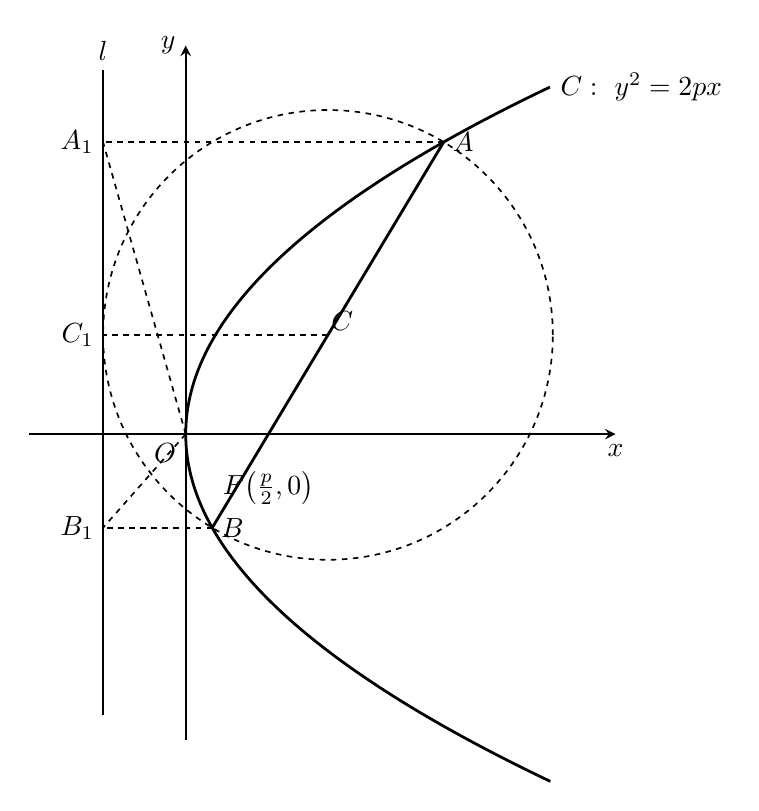
\begin{tikzpicture}[
%			scale=1.05, >=Latex,
			scale=1.05, >=stealth,
			point/.style={circle,fill=black,inner sep=1.3pt},
			axis/.style={->, line width=0.7pt},
			thin/.style={line width=0.7pt},
			chord/.style={line width=1.0pt},
			parab/.style={smooth, samples=220, line width=1.0pt},
			dashedthin/.style={dash pattern=on 2pt off 2pt, line width=0.6pt}
			]
			% =========================================================
			% 参数：抛物线 C: y^2 = 2 p x (p>0)
			% 取一条过焦点的弦 AB，其直线可设为 x = m y + p/2
			% 你只需要改 p 与 m，就能自动得到一张“标准焦点弦图”
			% =========================================================
			\def\p{2}      % p>0，可改
			\def\m{0.6}    % 可改（决定焦点弦的“倾斜程度”）
			
			% 计算若干关键量
			\pgfmathsetmacro{\fx}{\p/2}             % 焦点 F 的 x 坐标
			\pgfmathsetmacro{\dirx}{-\p/2}          % 准线 x=-p/2
			\pgfmathsetmacro{\s}{sqrt(\m*\m+1)}     % sqrt(m^2+1)
			
			% 交点 A,B：由 y^2 = 2p(m y + p/2) => y = p(m ± sqrt(m^2+1))
			\pgfmathsetmacro{\yA}{\p*(\m+\s)}
			\pgfmathsetmacro{\yB}{\p*(\m-\s)}
			\pgfmathsetmacro{\xA}{\m*\yA+\p/2}
			\pgfmathsetmacro{\xB}{\m*\yB+\p/2}
			
			% 中点 C
			\pgfmathsetmacro{\xC}{(\xA+\xB)/2}
			\pgfmathsetmacro{\yC}{(\yA+\yB)/2}
			
			% 以 AB 为直径的圆：圆心 C，半径 r=|AB|/2=|CC1|=p(m^2+1)
			\pgfmathsetmacro{\r}{\p*(\m*\m+1)}
			
			% 坐标点
			\coordinate (O)  at (0,0);
			\coordinate (F)  at (\fx,0);
			\coordinate (A)  at (\xA,\yA);
			\coordinate (B)  at (\xB,\yB);
			\coordinate (C)  at (\xC,\yC);
			\coordinate (A1) at (\dirx,\yA);
			\coordinate (B1) at (\dirx,\yB);
			\coordinate (C1) at (\dirx,\yC);
			
			% 坐标轴
			\draw[axis] (-1.9,0) -- (5.2,0) node[below] {$x$};
			\draw[axis] (0,-3.7) -- (0,4.7) node[left] {$y$};
			\node[below left] at (O) {$O$};
			
			% 抛物线：参数法 y=t, x=t^2/(2p)
			\draw[parab,domain=-4.2:4.2]
			plot ({(\x*\x)/(2*\p)}, {\x})
			node[right] {$C:\ y^{2}=2px$};
			
			% 准线 l: x=-p/2
			\draw[thin] (\dirx,-3.4) -- (\dirx,4.4) node[above] {$l$};
			
			% 焦点
			\draw[point] (F) node[below] {$F\!\left(\frac p2,0\right)$};
			
			% 焦点弦 AB
			\draw[chord] (A) -- (B);
			\draw[point] (A) node[right] {$A$};
			\draw[point] (B) node[right] {$B$};
			
			% 中点 C
			\draw[point] (C) node[above right] {$C$};
			
			% A,B,C 在准线上的射影 A1,B1,C1（垂直于准线，因此为水平虚线）
			\draw[dashedthin] (A) -- (A1);
			\draw[dashedthin] (B) -- (B1);
			\draw[dashedthin] (C) -- (C1);
			\draw[point] (A1) node[left] {$A_{1}$};
			\draw[point] (B1) node[left] {$B_{1}$};
			\draw[point] (C1) node[left] {$C_{1}$};
			
			% 连接 FA, FB（突出“过焦点弦”）
			\draw[thin] (F) -- (A);
			\draw[thin] (F) -- (B);
			
			% 性质常用共线：O,A,B1 共线；O,B,A1 共线（画出延长线）
			\draw[dashedthin] (O) -- (B1);
			\draw[dashedthin] (O) -- (A1);
			
			% 以 AB 为直径的圆（圆心 C，过 A,B），并与准线相切于 C1
			\draw[dashedthin] (C) circle (\r);
			\draw[dashedthin] (C) -- (C1);
			
		\end{tikzpicture}
	}
		\caption{抛物线 $y^{2}=2px$ 的焦点弦 $AB$：中点 $C$ 及其在准线上的射影 $A_1,B_1,C_1$}
	\end{figure}
	
	\section*{圆锥曲线的光学性质（抛物线、椭圆、双曲线）}
	
	\subsection*{0.\ 共同的几何本质（切线“平分角”观点）}
	
	
	
	
	
	\begin{itemize}
		\item \textbf{抛物线：} 切线平分“焦半径 $PF$”与“与轴平行方向”所成的角；
		\item \textbf{椭圆：} 切线平分 $PF_1$ 与 $PF_2$ 的\textbf{内角}；
		\item \textbf{双曲线：} 切线平分 $PF_1$ 与 $PF_2$ 的\textbf{外角}（等价地：反射光线的反向延长线过另一个焦点）。
	\end{itemize}
	这些结论也常用费马原理（光程取极值/驻值）来解释。
	
	\subsection*{1.\ 抛物线的光学性质（会聚与平行）}
	以
	\[
	C:\ y^2=2px\ (p>0),\quad F\left(\frac p2,0\right),\quad l:\ x=-\frac p2
	\]
	为例：
	\begin{itemize}
		\item 任意\textbf{平行于轴}的入射光线照到抛物线后，反射光线\textbf{必过焦点 $F$}；
		\item 反过来，从焦点 $F$ 发出的光线照到抛物线后，反射光线\textbf{必与轴平行}（形成平行光束）。
	\end{itemize}
	
	\begin{figure}[htbp]
		\centering
		\begin{tikzpicture}[scale=0.95,>=stealth,
			point/.style={circle,fill=black,inner sep=1.2pt},
			thin/.style={line width=0.7pt},
			parab/.style={smooth,samples=180,line width=1.0pt},
			]
			\def\p{2} % 取 p=2，则 y^2=4x
			\coordinate (O) at (0,0);
			\coordinate (F) at ({\p/2},0);
			\draw[->] (-1.6,0)--(4.2,0) node[below] {$x$};
			\draw[->] (0,-2.8)--(0,3.2) node[left] {$y$};
			\node[below left] at (O) {$O$};
			
			% 准线 x=-p/2
			\draw[thin] ({-\p/2},-2.6)--({-\p/2},3.0) node[above] {$l:\ x=-\frac p2$};
			
			% 抛物线 y^2=2px：参数 y=t, x=t^2/(2p)
			\draw[parab,domain=-2.6:2.6] plot ({(\x*\x)/(2*\p)},{\x})
			node[right] {$C:\ y^2=2px$};
			
			% 取一点 P 在抛物线上（例如 y0=2）
			\coordinate (P) at ({(2*2)/(2*\p)},2); % x= y^2/(2p)
			\draw[point] (P) node[right] {$P$};
			
			% 焦点
			\draw[point] (F) node[below] {$F$};
			
			% 切线：y y0 = p(x+x0)，这里 y0=2,x0=1,p=2 => y=x+1
			\draw[thin] (-1.2,-0.2)--(3.6,4.6);
			\node[right] at (3.2,4.3) {$t_P$};
			
			% 入射光：平行于轴（水平）
			\draw[->,thin] (-1.0,2)--(P);
			
			% 反射光：过焦点
			\draw[->,thin] (P)--(F);
			
			% 说明文字
			\node at (2.4,-2.2) {$\text{平行光}\ \Rightarrow\ \text{反射过焦点}$};
		\end{tikzpicture}
		\caption{抛物线的反射性质：平行于轴的入射光线经反射通过焦点（逆命题同样成立）}
	\end{figure}
	
	\subsection*{2.\ 椭圆的光学性质（两焦点互相“成像”）}
	以椭圆
	\[
	E:\ \frac{x^2}{a^2}+\frac{y^2}{b^2}=1\ (a>b>0),\qquad
	F_1(-c,0),\ F_2(c,0),\ c^2=a^2-b^2
	\]
	为例：
	\begin{itemize}
		\item 从一个焦点 $F_1$ 发出的光线射到椭圆上任一点 $P$，按反射定律反射后\textbf{必通过另一个焦点 $F_2$}；
		\item 等价表述：在 $P$ 处的切线 $t_P$ 平分 $\angle F_1PF_2$ 的\textbf{内角}。
	\end{itemize}
	
	\begin{figure}[htbp]
		\centering
		\begin{tikzpicture}[scale=0.9,>=stealth,
			point/.style={circle,fill=black,inner sep=1.2pt},
			thin/.style={line width=0.7pt},
			conic/.style={smooth,samples=240,line width=1.0pt},
			dashedthin/.style={dash pattern=on 2pt off 2pt, line width=0.6pt},
			]
			% 取参数
			\def\a{4.0}
			\def\b{2.5}
			\pgfmathsetmacro{\c}{sqrt(\a*\a-\b*\b)}
			\def\t{50} % 取点参数角
			
			% 坐标轴
			\draw[->] (-4.8,0)--(4.8,0) node[below] {$x$};
			\draw[->] (0,-3.4)--(0,3.6) node[left] {$y$};
			
			% 椭圆：x=a cos t, y=b sin t
			\draw[conic,domain=0:360] plot ({\a*cos(\x)},{\b*sin(\x)})
			node[right] {$\frac{x^2}{a^2}+\frac{y^2}{b^2}=1$};
			
			% 焦点
			\coordinate (F1) at (-\c,0);
			\coordinate (F2) at (\c,0);
			\draw[point] (F1) node[below] {$F_1$};
			\draw[point] (F2) node[below] {$F_2$};
			
			% 点 P
			\coordinate (P) at ({\a*cos(\t)},{\b*sin(\t)});
			\draw[point] (P) node[above right] {$P$};
			
			% 连接焦点到P，并画“反射路径”：F1->P->F2
			\draw[->,thin] (F1)--(P);
			\draw[->,thin] (P)--(F2);
			
			% 切线方向（参数导数方向）：(-a sin t, b cos t)
			\pgfmathsetmacro{\dx}{-\a*sin(\t)}
			\pgfmathsetmacro{\dy}{\b*cos(\t)}
			\coordinate (Pd) at ({\a*cos(\t)+\dx},{\b*sin(\t)+\dy});
			\draw[dashedthin] ($(P)!-0.30!(Pd)$)--($(P)!0.30!(Pd)$) node[right] {$t_P$};
			
			\node at (0,-3.0) {$\text{从 }F_1\text{ 出发}\Rightarrow\text{反射后过 }F_2$};
		\end{tikzpicture}
		\caption{椭圆的反射性质：从一个焦点出发的光线，经椭圆反射后通过另一个焦点（切线平分内角）}
	\end{figure}
	
	\subsection*{3.\ 双曲线的光学性质（“虚焦点”现象）}
	以双曲线
	\[
	H:\ \frac{x^2}{a^2}-\frac{y^2}{b^2}=1\ (a,b>0),\qquad
	F_1(-c,0),\ F_2(c,0),\ c^2=a^2+b^2
	\]
	为例（只画右支）：
	\begin{itemize}
		\item 设光线从焦点 $F_1$ 射向右支上一点 $P$，反射后得到一条出射光线；
		则\textbf{出射光线的反向延长线必经过另一个焦点 $F_2$}（因此常说 $F_2$ 是“虚焦点”）；
		\item 等价表述：在 $P$ 处切线 $t_P$ 平分 $\angle F_1PF_2$ 的\textbf{外角}。
	\end{itemize}
	
	\begin{figure}[htbp]
		\centering
		\begin{tikzpicture}[scale=0.9,>=stealth,
			point/.style={circle,fill=black,inner sep=1.2pt},
			thin/.style={line width=0.7pt},
			conic/.style={smooth,samples=260,line width=1.0pt},
			dashedthin/.style={dash pattern=on 2pt off 2pt, line width=0.6pt},
			]
			% 参数
			\def\a{3.0}
			\def\b{2.0}
			\pgfmathsetmacro{\c}{sqrt(\a*\a+\b*\b)}
			\def\t{35} % 参数角（用 sec,tan 参数）
			
			% 坐标轴
			\draw[->] (-5.2,0)--(6.2,0) node[below] {$x$};
			\draw[->] (0,-4.2)--(0,4.2) node[left] {$y$};
			
			% 渐近线 y=±(b/a)x
			\draw[dashedthin] (-5.0,{-\b/\a*5.0})--(5.6,{\b/\a*5.6});
			\draw[dashedthin] (-5.0,{\b/\a*5.0})--(5.6,{-\b/\a*5.6});
			
			% 右支参数：x=a sec t, y=b tan t
			\draw[conic,domain=-70:70]
			plot ({\a/cos(\x)},{\b*tan(\x)})
			node[right] {$\frac{x^2}{a^2}-\frac{y^2}{b^2}=1$};
			
			% 焦点
			\coordinate (F1) at (-\c,0);
			\coordinate (F2) at (\c,0);
			\draw[point] (F1) node[below] {$F_1$};
			\draw[point] (F2) node[below] {$F_2$};
			
			% 点 P
			\coordinate (P) at ({\a/cos(\t)},{\b*tan(\t)});
			\draw[point] (P) node[above right] {$P$};
			
			% 入射：F1 -> P
			\draw[->,thin] (F1)--(P);
			
			% 出射：沿直线 PF2 的反方向离开（反向延长线过 F2）
			\draw[dashedthin] (P)--(F2); % 反向延长线（虚线）
			\draw[->,thin] (P)--($(P)!-0.55!(F2)$); % 真正出射方向：背离 F2
			
			% 切线方向：由 y' = b^2 x / (a^2 y)，可取方向向量 (a^2 y0, b^2 x0)
			\pgfmathsetmacro{\xP}{\a/cos(\t)}
			\pgfmathsetmacro{\yP}{\b*tan(\t)}
			\pgfmathsetmacro{\dx}{\a*\a*\yP}
			\pgfmathsetmacro{\dy}{\b*\b*\xP}
			\coordinate (Pd) at ({\xP+\dx},{\yP+\dy});
			\draw[dashedthin] ($(P)!-0.18!(Pd)$)--($(P)!0.18!(Pd)$) node[right] {$t_P$};
			
			\node at (0,-3.6) {$\text{出射光线反向延长线过 }F_2\ (\text{外角平分})$};
		\end{tikzpicture}
		\caption{双曲线的反射性质：从 $F_1$ 指向右支的入射光，反射后其反向延长线经过 $F_2$（“虚焦点”）}
	\end{figure}
	
	\subsection*{4.\ 补充：圆的情形（椭圆的特例）}
	圆可看作椭圆的特例（两焦点重合）。圆的镜面反射中，\textbf{法线恒过圆心}；
	因此从圆心射向圆周的光线总是沿半径入射并沿原路反射返回。
	
\end{document}
